\chapter{Discusión}

\section{Qué cambia respecto del diagnóstico del FMI}

El FMI (2026) concluye que la deuda argentina es sostenible pero no con
alta probabilidad, y estima en 1\% la probabilidad de que no se
estabilice en el mediano plazo. Esta tesis mide la misma deuda desde el
mismo punto de partida, con el mismo escenario, horizonte y métrica, y
obtiene 32,8\% en 2031. Como todo lo demás coincide, la distancia tiene
que venir de la distribución de los \emph{shocks} aplicados al
escenario.

El procedimiento del FMI aplicado a la historia argentina de 2000-2025
tampoco reproduce el 1\%: da 16,6\%. El FMI no publica la historia de
\emph{shocks} con la que arma su abanico para Argentina, de modo que la
tesis no puede saber qué lo hace tan benigno y no atribuye la brecha a
una causa que no puede verificar. El propio marco del FMI advierte que
sus abanicos subestiman la incertidumbre, porque omiten la
retroalimentación de la deuda y fijan la composición por monedas (FMI,
2021, anexo VI, párr. 6). La retroalimentación, de todos modos, explica
poco de la distancia entre el SVARX y el procedimiento del FMI: sin
ella, la probabilidad del SVARX apenas cambia (Apéndice, sección A.8).

\textbf{Federal y consolidada.} Consolidar con el BCRA baja el punto de
partida a 52,1\% del PIB. Su proporción en moneda extranjera es mayor,
pero la deuda en moneda extranjera medida en puntos del PIB es menor, y
con menos deuda expuesta a la tasa en dólares y a la depreciación real
la probabilidad de no estabilización baja a 26,8\% en 2031. La dinámica
estimada con la serie consolidada se parece a la federal: la reacción
fiscal es algo mayor, con intervalos que se superponen (Tabla 6.1), y
las tres hipótesis llevan a las mismas conclusiones. La consolidación
aporta, sobre todo, una medición distinta del \emph{stock} expuesto a
los \emph{shocks}.

\section{Por qué el abanico es más angosto y, aun así, la probabilidad
es mayor}

El abanico del SVARX mide 48,3 puntos del PIB en 2031, contra 71,5 del
FMI y 151,1 del procedimiento del FMI aplicado a la historia argentina,
que comparte con el SVARX deuda, identidad y métrica (Figura 7.1).

\begin{figure}
\centering
\pandocbounded{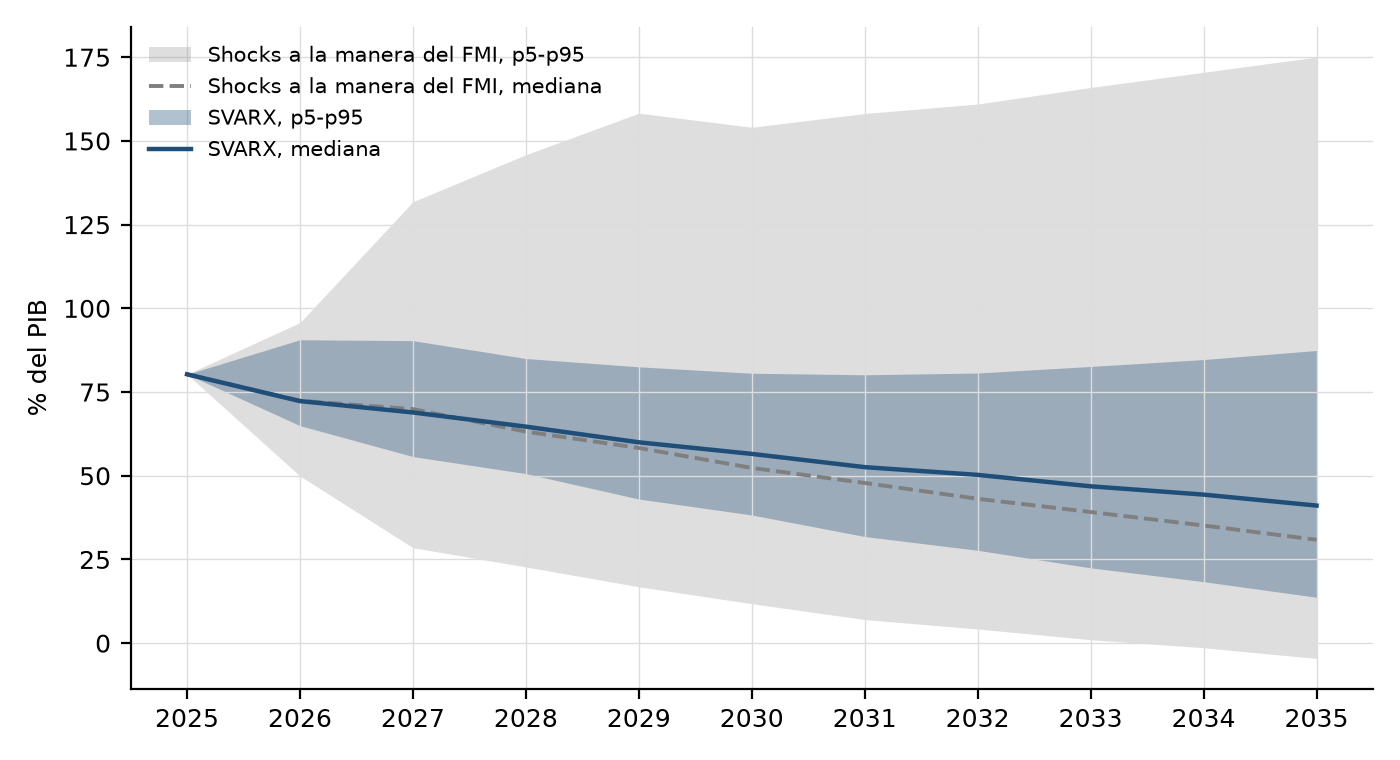
\includegraphics[keepaspectratio,alt={Abanicos con shocks del SVARX y con shocks a la manera del FMI. Deuda federal bruta simulada, percentiles 5 y 95 y mediana (\% del PIB); los shocks a la manera del FMI son bloques de dos años de desvíos históricos de los impulsores anuales, 2000-2025. Fuente: elaboración propia.}]{fig7_1_abanico_svarx_vs_fmi.png}}
\caption[Abanicos con \emph{shocks} del SVARX y con \emph{shocks} a la manera del FMI]{Abanicos con \emph{shocks} del SVARX y con \emph{shocks} a la
manera del FMI. Deuda federal bruta simulada, percentiles 5 y 95 y
mediana (\% del PIB); los \emph{shocks} a la manera del FMI son bloques
de dos años de desvíos históricos de los impulsores anuales, 2000-2025.
Fuente: elaboración propia.}
\end{figure}

El procedimiento del FMI mide los \emph{shocks} como desvíos de cada
impulsor respecto de una única media, y la historia argentina reúne
regímenes monetarios muy distintos (Figura 7.2). Es el riesgo que el FMI
y el Mecanismo Europeo de Estabilidad (2023) señalan en su método: que
la historia usada no sea representativa del futuro. La Tabla 7.1 repite
la variante quitando 2002 o fijando cada impulsor en su media.

\begin{figure}
\centering
\pandocbounded{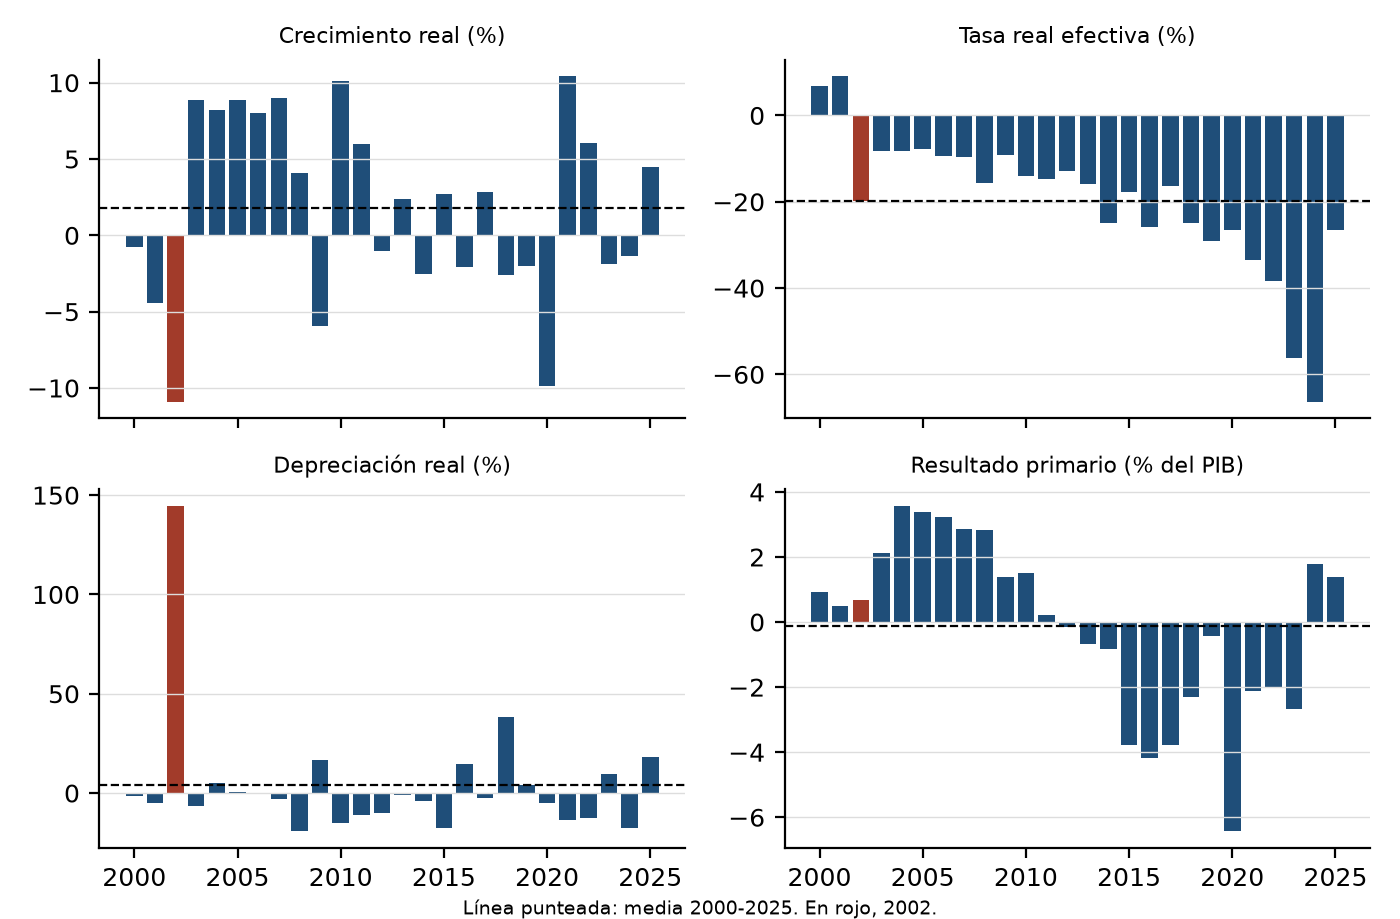
\includegraphics[keepaspectratio,alt={Impulsores anuales de la deuda, 2000-2025. Crecimiento real, tasa real efectiva, depreciación real y resultado primario que usa la variante a la manera del FMI; la línea punteada es la media del período y en rojo se marca 2002. Fuente: elaboración propia.}]{fig7_2_impulsores_historicos.png}}
\caption[Impulsores anuales de la deuda, 2000-2025]{Impulsores anuales de la deuda, 2000-2025. Crecimiento real,
tasa real efectiva, depreciación real y resultado primario que usa la
variante a la manera del FMI; la línea punteada es la media del período
y en rojo se marca 2002. Fuente: elaboración propia.}
\end{figure}

\textbf{Tabla 7.1. Diagnóstico de la variante con \emph{shocks} a la
manera del FMI (deuda federal bruta)}

{\def\LTcaptype{none} % do not increment counter
\begin{longtable}[]{@{}
  >{\raggedright\arraybackslash}p{(\linewidth - 6\tabcolsep) * \real{0.2500}}
  >{\raggedright\arraybackslash}p{(\linewidth - 6\tabcolsep) * \real{0.2500}}
  >{\raggedright\arraybackslash}p{(\linewidth - 6\tabcolsep) * \real{0.2500}}
  >{\raggedright\arraybackslash}p{(\linewidth - 6\tabcolsep) * \real{0.2500}}@{}}
\toprule\noalign{}
\begin{minipage}[b]{\linewidth}\raggedright
Variante
\end{minipage} & \begin{minipage}[b]{\linewidth}\raggedright
No estabilización 2031
\end{minipage} & \begin{minipage}[b]{\linewidth}\raggedright
No estabilización 2035
\end{minipage} & \begin{minipage}[b]{\linewidth}\raggedright
Ancho del abanico 2031
\end{minipage} \\
\midrule\noalign{}
\endhead
\bottomrule\noalign{}
\endlastfoot
Todos los años, 2000-2025 & 16,6\% & 15,1\% & 151,1 \\
Sin el año 2002 & 23,6\% & 21,4\% & 104,3 \\
Depreciación real en su media & 17,6\% & 18,6\% & 102,0 \\
Tasa real efectiva en su media & 20,4\% & 18,4\% & 97,8 \\
Crecimiento en su media & 29,1\% & 23,7\% & 128,3 \\
Resultado primario en su media & 16,7\% & 15,0\% & 153,4 \\
\end{longtable}
}

Fuente: elaboración propia. 20.000 trayectorias por variante, con los
mismos números aleatorios que la Tabla 6.6.

Quitar 2002 achica el abanico en un tercio, y fijar en su media la
depreciación real o la tasa real lo achica más todavía; la probabilidad,
en cambio, sube. El ancho lo determinan unos pocos años extremos. Los
\emph{shocks} de este procedimiento son desvíos respecto de la media
histórica. Sin 2002, la depreciación real media pasa de 4,0\% a -1,6\% y
la proporción de años con depreciación por encima de la media sube de
31\% a 44\%: el abanico pierde su cola extrema pero gana desvíos
desfavorables moderados, que activan la métrica más seguido. Fijar un
impulsor en su media tiene otro efecto: elimina también sus desvíos
favorables, que en la historia compensaban a los demás. El crecimiento,
por ejemplo, tiene una correlación de -0,51 con la depreciación real y
de 0,44 con el resultado primario.

Lo mismo explica la diferencia con el SVARX. El SVARX trata los cambios
de régimen con los quiebres, remuestrea solo las sorpresas, que son
menores que los desvíos respecto de una media de largo plazo, y reprecia
la tasa en dólares a medida que vence la deuda; por eso su abanico es
más angosto. La métrica del FMI, sin embargo, no mira la dispersión
acumulada: compara en el año T el resultado primario previsto con el que
estabilizaría la deuda ese año, un umbral que se mueve con la tasa
efectiva, el crecimiento y la valuación de la deuda en moneda extranjera
de un solo año. El SVARX conserva esa volatilidad anual, y con más de la
mitad de la deuda en moneda extranjera basta un año de depreciación real
o de crecimiento bajo para que el resultado necesario supere al
previsto, aunque la deuda siga bajando.

\section{El papel del superávit primario}

El resultado primario respondió a la deuda en 2000-2025, como pide la
condición de Bohn (1998), pero el bloque fiscal explica menos de una
décima parte de la varianza de la deuda en 2035, y los bloques externo y
cambiario y de riesgo, cerca de cuatro quintos. La conclusión no depende
de la identificación: aun cuando el \emph{shock} fiscal absorbe toda la
covarianza con el crecimiento, la diferencia a favor de los
\emph{shocks} no fiscales excluye el cero. Una depreciación real o una
suba de la tasa en dólares cambian el cociente de deuda aunque las
cuentas fiscales estén en orden (Calvo et al., 2003).

El análisis de suficiencia lo ilustra desde otro ángulo. Un superávit
igual al del mejor año desde 1999, sostenido toda la década, deja sin
estabilizar la deuda de 2031 en una de cada cuatro trayectorias, y
llevar la probabilidad a la cifra del FMI exigiría un superávit cercano
al 10\% del PIB, sin precedentes en la historia argentina. El superávit
es necesario, y el escenario del FMI se apoya en él, pero no controla
las fuentes de riesgo que dominan la varianza.

\section{\texorpdfstring{El \emph{shock} de la FED}{El shock de la FED}}

H2 queda respaldada en su efecto y no en su mecanismo. Repetir la senda
de la tasa de la FED de 2022-2025 eleva la probabilidad de no
estabilización en 2035, y el efecto resiste la corrección por contrastes
múltiples y casi todas las especificaciones. El efecto sobre la deuda
esperada es menos firme: no resiste Bonferroni y se sostiene en menos de
dos tercios de las especificaciones.

Tres cuartos del aumento de la deuda vienen del mayor costo de la deuda
en dólares, que el modelo incorpora por construcción a través de la
identidad. Los canales que nombra la hipótesis no se distinguen del
azar, y las pocas respuestas significativas, del tipo de cambio real,
tienen el signo contrario al esperado. Uribe y Yue (2006) y Canova
(2005) documentan esos canales con paneles y muestras más largas; una
sola serie argentina de 102 trimestres no alcanza para medirlos. El
bloque externo es, aun así, el de mayor participación en la varianza de
la deuda: la tasa de la FED y el VIX importan para la incertidumbre
aunque sus canales no se puedan separar.

\section{Diálogo con la literatura}

\begin{itemize}
\tightlist
\item
  \textbf{Balance patrimonial.} Levy Yeyati y Sturzenegger (2023)
  encuentran que una devaluación real de 20\% casi no modifica el
  patrimonio neto del sector público argentino, porque el mayor costo de
  la deuda en dólares se compensa con más recaudación de bienes
  transables. Esta tesis mide el cociente de deuda, cuya varianza
  dominan los \emph{shocks} cambiarios, de riesgo y externos. Las dos
  conclusiones son compatibles: el cociente puede no estabilizarse
  aunque el patrimonio neto se mantenga, y por eso Rodríguez (2023)
  advierte que es una medida engañosa después de un salto cambiario.
\item
  \textbf{Tasa y crecimiento.} Blanchard (2019) muestra que, con una
  tasa de interés menor que el crecimiento, la deuda se licua sin
  necesidad de superávit. El escenario del FMI tiene esa propiedad toda
  la década, y la mediana simulada baja en consecuencia; la licuación,
  sin embargo, no garantiza la estabilización año por año con una parte
  grande de la deuda en moneda extranjera.
\item
  \textbf{Fatiga fiscal.} Ghosh et al.~(2013) sostienen que la respuesta
  del superávit se debilita con deuda alta, y Everaert y Jansen (2018)
  no lo confirman. La regla lineal de esta tesis no permite
  contrastarlo.
\end{itemize}

\section{Limitaciones}

\begin{itemize}
\tightlist
\item
  \textbf{Escenario base.} Los resultados están condicionados al
  escenario del FMI, tomado como dado, con una tasa real efectiva
  negativa y un superávit sostenido; si la desinflación es más rápida,
  la licuación se reduce.
\item
  \textbf{Retroalimentación anual.} La deuda vuelve al sistema al cierre
  de cada año; dentro del año, las ecuaciones usan la del cierre
  anterior.
\item
  \textbf{Composición por monedas fija.} Si la depreciación real eleva
  la proporción en moneda extranjera, el riesgo cambiario está
  subestimado, como en el FMI.
\item
  \textbf{Variables externas.} Los procesos AR(1) del VIX y de la FED no
  se reestiman en cada réplica del \emph{bootstrap}, y el VIX no
  responde a la FED.
\item
  \textbf{Quiebres.} Sus fechas se estiman sobre la serie de deuda y se
  toman como conocidas; solo mueven el nivel de las ecuaciones, y el
  régimen posterior a 2024 casi no está en la muestra.
\item
  \textbf{Muestra y normalidad.} Con 102 trimestres, los efectos de la
  FED y de la retroalimentación tienen intervalos amplios. Los residuos
  rechazan la normalidad; el remuestreo evita suponerla, pero la
  inferencia descansa en el \emph{bootstrap}.
\item
  \textbf{Extensión consolidada.} Usa el escenario del FMI construido
  para la deuda federal, con el ajuste stock-flujo y la inflación
  relativa escalados, y su serie histórica no descuenta los títulos en
  poder del FGS.
\item
  \textbf{\emph{Shock} de la FED.} Es la variación observada de la tasa
  y no un \emph{shock} monetario identificado con datos de alta
  frecuencia.
\end{itemize}
